% trefoil_vs_unknot.tex — (2,3) phase-space trefoil vs 0_1 real-space unknot (Vol 9 Ch.11)
% Pure TikZ (no pgfplots): hardens INVARIANT-N1 — the electron's PHASE-SPACE winding portrait
% is the (2,3) trefoil on the Clifford torus; its REAL-SPACE body is the 0_1 unknot.
\begin{figure}[htbp]
\centering
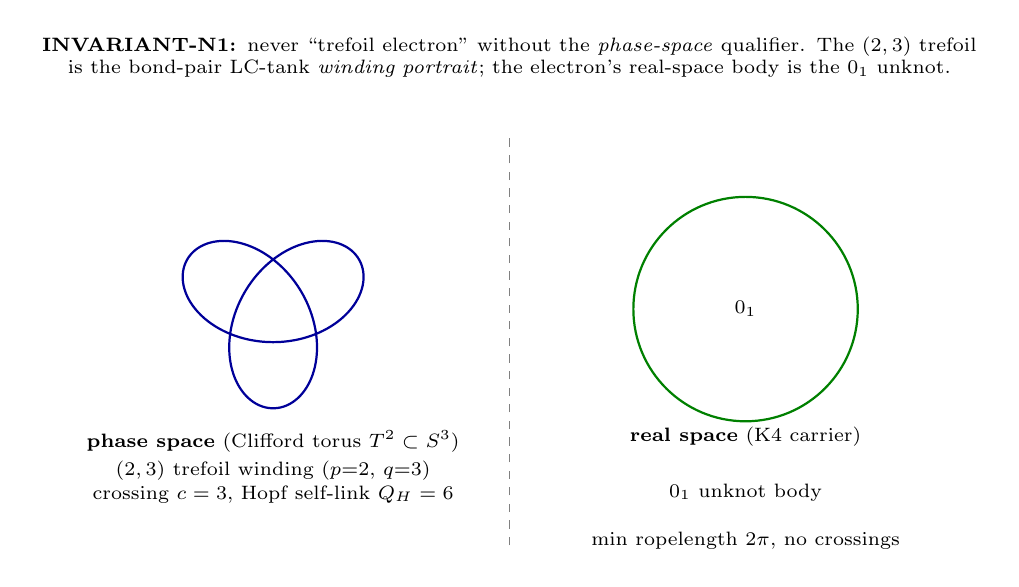
\begin{tikzpicture}[
    kcap/.style={font=\scriptsize, align=center},
    note/.style={font=\scriptsize, align=center}
]
    % ---- LEFT: (2,3) phase-space trefoil on the Clifford torus ----
    % parametric trefoil: x = sin t + 2 sin 2t, y = cos t - 2 cos 2t  (scaled)
    \begin{scope}[shift={(0,0)}, scale=0.42]
        \draw[thick, blue!60!black, domain=0:360, samples=200, smooth, variable=\t]
            plot ({sin(\t) + 2*sin(2*\t)}, {cos(\t) - 2*cos(2*\t)});
        \node[kcap] at (0,-4.0) {\textbf{phase space} (Clifford torus $\mathbb{T}^2 \subset S^3$)};
        \node[kcap] at (0,-4.9) {$(2,3)$ trefoil winding ($p{=}2$, $q{=}3$)};
        \node[kcap] at (0,-5.6) {crossing $c = 3$, Hopf self-link $Q_H = 6$};
    \end{scope}

    % divider
    \draw[gray, dashed] (3.0,-3.0) -- (3.0,2.2);

    % ---- RIGHT: 0_1 real-space unknot (plain loop) ----
    \begin{scope}[shift={(6.0,0)}, scale=0.95]
        \draw[thick, green!50!black] (0,0) circle (1.5);
        \node[note] at (0,0) {$0_1$};
        \node[kcap] at (0,-1.7) {\textbf{real space} (K4 carrier)};
        \node[kcap] at (0,-2.45) {$0_1$ unknot body};
        \node[kcap] at (0,-3.1) {min ropelength $2\pi$, no crossings};
    \end{scope}

    % discipline banner
    \node[note, text width=12.0cm] at (3.0,3.2)
        {\textbf{INVARIANT-N1:} never ``trefoil electron'' without the \emph{phase-space} qualifier. The $(2,3)$ trefoil is the bond-pair LC-tank \emph{winding portrait}; the electron's real-space body is the $0_1$ unknot.};
\end{tikzpicture}
\caption{Phase-space winding vs real-space body (Vol.~9 Ch.~11 \S\ref{sec:vol9_torus_knot_winding}; disambiguation per INVARIANT-N1). Left: the electron's $(2,3)$ trefoil winding portrait on the Clifford torus $\mathbb{T}^2 \subset S^3 \subset \mathbb{C}^2$ (phase-space coordinates per \texttt{phase-space-coordinate-check}). Right: the electron's real-space body, the $0_1$ unknot on the K4 carrier (the simplest closed flux-tube loop, no crossings). The two are distinct coordinate systems, both substrate-native primary; conflating them is the ``trefoil electron'' misread. Canonical at \kbleaf{electron-unknot.md} + \kbleaf{torus-knot-uniqueness.md} (\texttt{clm-8c3yhs}).}
\label{fig:vol9_trefoil_vs_unknot}
\end{figure}
